% !TeX root = ../main.tex
\section{Sensor Networks and Simplicial Complexes} % (fold)
\label{sec:complexes}

We consider the problem of determining coverage in a coordinate free sensor network.
That is, we would like to determine if an unknown domain is covered by a collection of sensors without their precise coordinates.
Let $\D$ denote our unknown domain and $P\subset\D$ be a collection of points, each representing a sensor in our network.
At the very least each sensor is capable of detecting nodes which are sufficiently ``close'' in the sense that, if we endow our domain with a metric $\dist:\D\times\D\to\R$ there is some radius of communication $\alpha > 0$ such that two nodes $p, q\in P$ such that $\dist(p, q) \leq\alpha$ are capable of communication.
Note that, although sensors can communicate within this distance they are not able to measure the distance itself.

With this limited capability we can construct an undirected graph $G=(V,E)$ with vertices $V=P$ and edges $E = \{\{p, q\}\subset P\mid \dist(p,q)\leq\alpha\}$.
In order to determine coverage we must at least assert that the coverage domain spanned by the points in $P$ does not contain any holes.
Assuming the coverage radius of our sensors is equal to their communication radius $\alpha$ we may define a hole in coverage as a cycle that cannot be ``filled'' with triangles.
This leads us to a more natural construction known as a simplicial complex.
\begin{definition}
   A \textbf{simplicial complex} $K$ is a collection of subsets, called \textbf{simplices}, of a vertex set $V$ such that for all $\sigma\in K$ and $\tau\subset\sigma$ it must follow that $\tau\in K$.
\end{definition}
The \textbf{dimension} of a simplex $\sigma\in K$ is defined as $\dim(\sigma) := |\sigma|-1$ where $|\cdot|$ denotes set cardinality.
The dimension of a simplicial complex $K$ is the maximum dimension of any simplex in $K$.
That is, a graph is a 1-dimensional simplicial complex in which vertices and edges are 0 and 1-dimensional simplices, respectively.

\begin{figure}[htbp]
\centering
    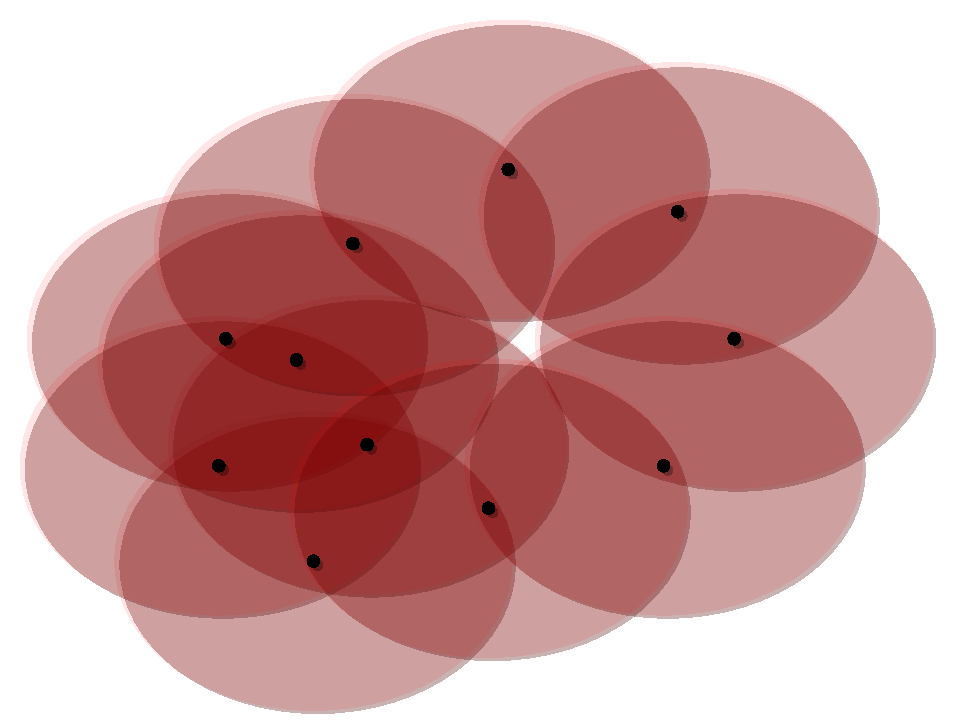
\includegraphics[scale=0.33]{figures/holes_cover.pdf}
    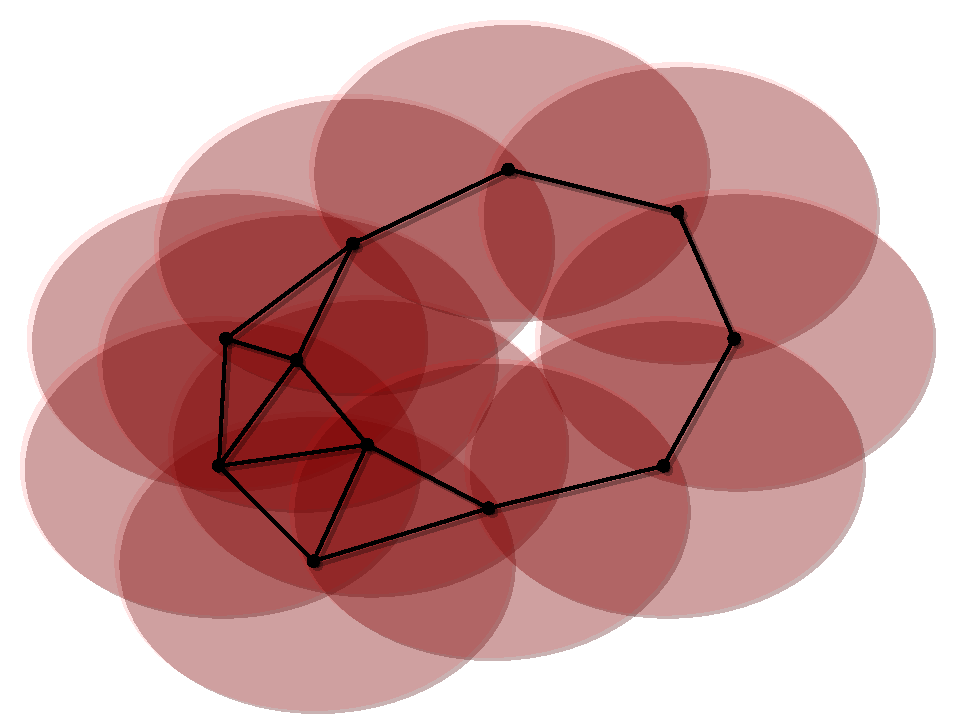
\includegraphics[scale=0.33]{figures/holes_edges.pdf}
    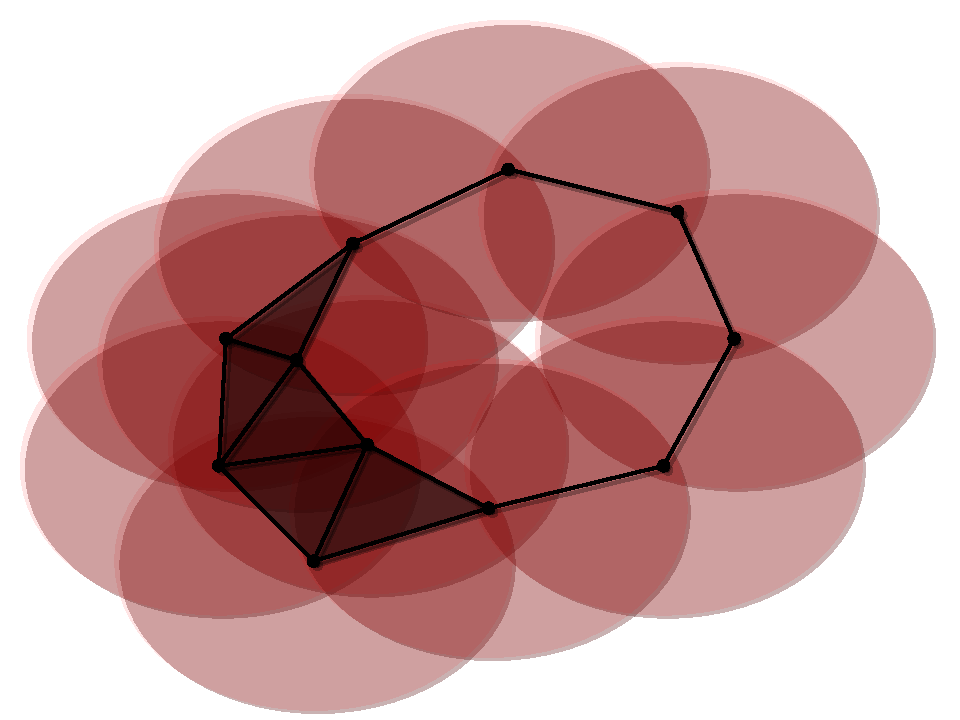
\includegraphics[scale=0.33]{figures/holes_complex.pdf}
     \caption{(Left) The coverage regions of a collection of points $P$ at some scale $\alpha$.
            (Middle) The neighborhood graph with edges for each pair of points within pairwise distance $\alpha$.
            (Right) If we attempt to fill cycles in the graph with triangles identify a cycle that cannot be filled which reflects a gap in coverage}
     \label{fig:holes}
 \end{figure}

It is natural to think of a $k$-dimensional simplicial complex as the generalization of an undirected graph consisting of vertices and edges, collections of at most 2 vertices, to collections of sets of at most $k-1$ vertices.
Just as we have defined a hole in our graph $G$ as a cycle that cannot be filled with triangles, we define a $k$-dimensinal hole in a simplicial complex as a $k$-cycle that cannot be filled with $(k+1)$-simplices.
In the next section we will formally define $k$-cycles and introduce simplicial homology as a tool for identifying when and which cycles cannot be filled.

% As such, simplicial complexes serve offer a more robust discrete representation of high dimensional domains.
Let $K$ be a simplicial complex with 0-simplices $\{v\}$ for all $p\in P$, 1-simpices $\{u, v\}\subset P$ for each edge in $E$, and 2-simplices $\{u,v,w\}\subset P$ whenever $\{\{\{u,v\},\{v,w\},\{u,w\}\}\subset E$.
This particular simplicial complex is known as the Vietoris-Rips complex.
\begin{definition}
    The \textbf{(Vietoris-)Rips complex} is defined for a set $P$ at scale $\e > 0$ as
    \[ \rips^\e(P) = \left\{\sigma \subseteq P\mid \forall p,q\in\sigma,\ \dist(p, q)\leq\e\right\}. \]
\end{definition}
% This construction generalizes to higher dimensions, allowing us to identify not only holes in planar graphs, ``holes'' in any dimension $k$ as $(k-1)$-cycles in high dimensional simplicial complexes.

 % \begin{figure}[htbp]
 % \centering
 %     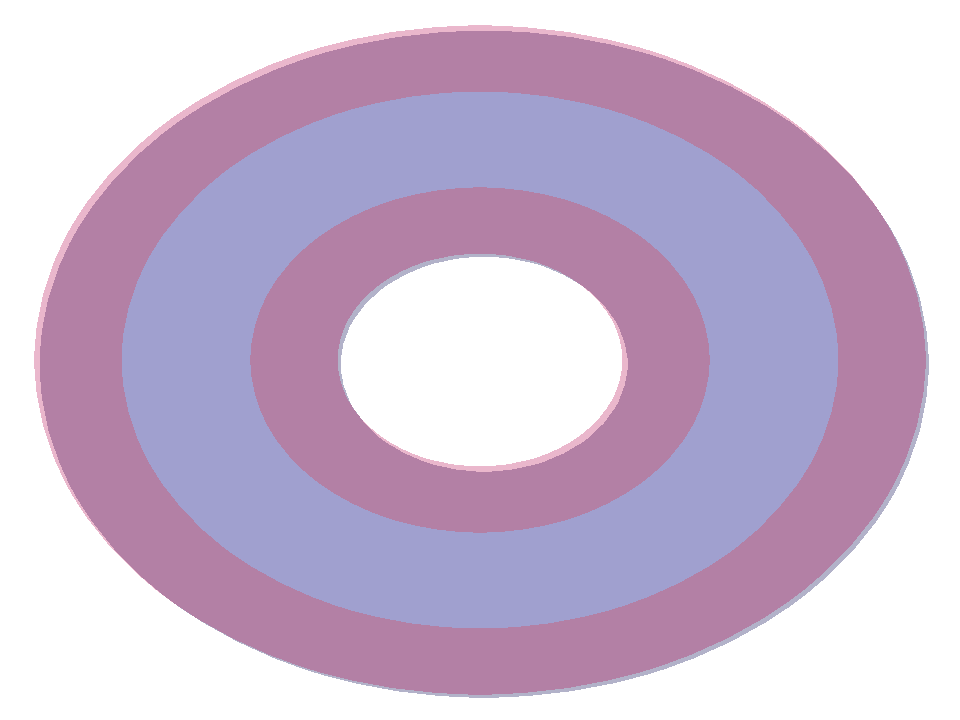
\includegraphics[scale=0.5]{figures/boundary_domain.pdf}
 %     % 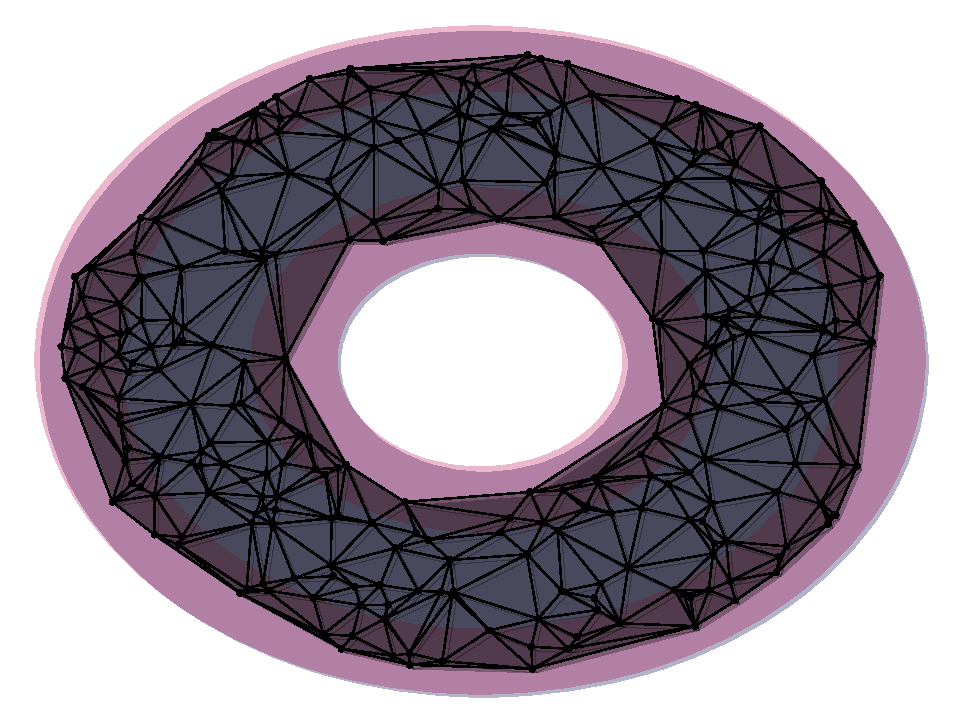
\includegraphics[scale=0.5]{figures/boundary_complex_domain.pdf}
 %     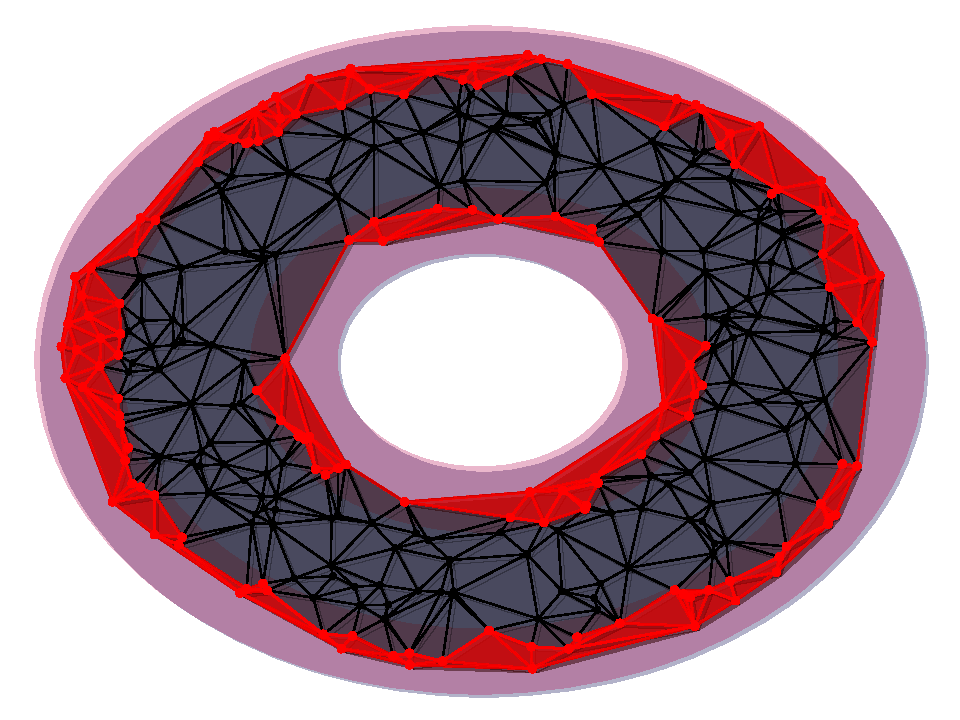
\includegraphics[scale=0.5]{figures/boundary_complex_domain_fence.pdf}
 %     % 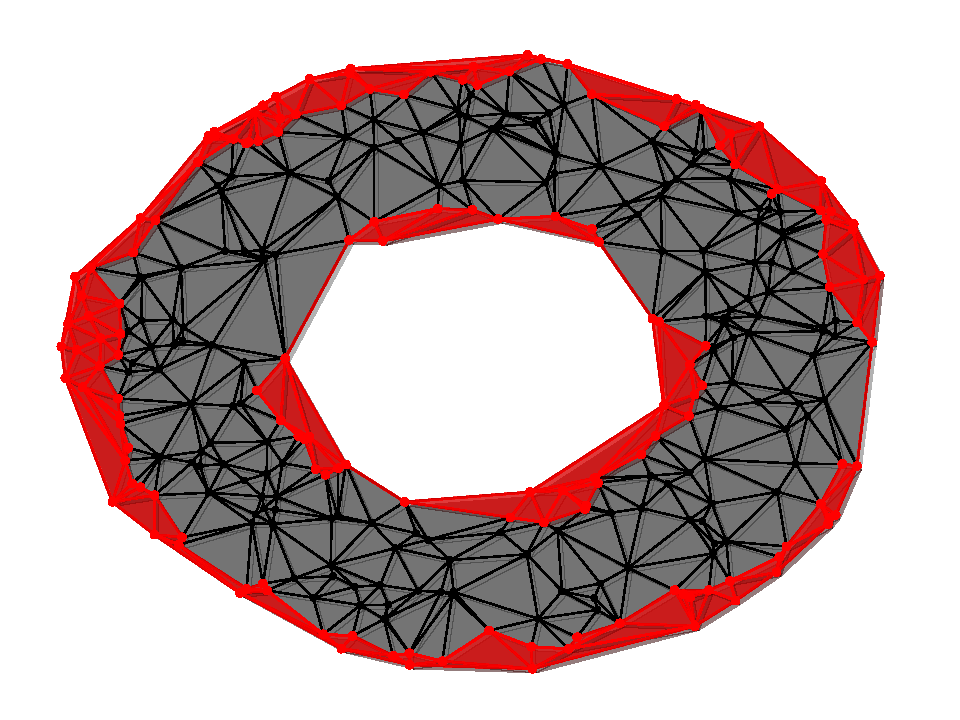
\includegraphics[scale=0.24]{figures/boundary_complex_fence.pdf}
 %      \caption{}
 %      \label{fig:boundary2}
 %  \end{figure}

\subsection{Coverage}

A subset $D$ of an domain $\D$ is covered by $P\subset$ at scale $\e > 0$ if every point $x\in D$ is within distance $\alpha$ at least one point in $P$.
\begin{definition}
    The \textbf{coverage region} of a point $p\in P$ at scale $\e > 0$ is defined
    \[\ball_\e(p) = \{x\in\D\mid \dist(x, p)\}.\]
\end{definition}
Let $P^\e$ to denote set of points in $\D$ within distance $\e$ of at least one point in $P$:
\[ P^\e = \bigcup_{p\in P}\ball_\e(p). \]
\begin{definition}
    Let $D, P\subset\D$.
    $D$ is \textbf{covered} by $P$ at scale $\e$ if $D\subseteq P^\e$.
\end{definition}
For this section we will assume that the coverage radius of our sensor network is equal to the radius of communication.
With this assumption we know that the converse problem is true: if a sensor network $P$ covers a domain at scale $\alpha$ the topology of the domain is reflected in $\rips^\alpha(P)$ however, as we will see this is in no way a tight bound on the minimal radius for coverage.

\begin{figure}[htbp]
\centering
    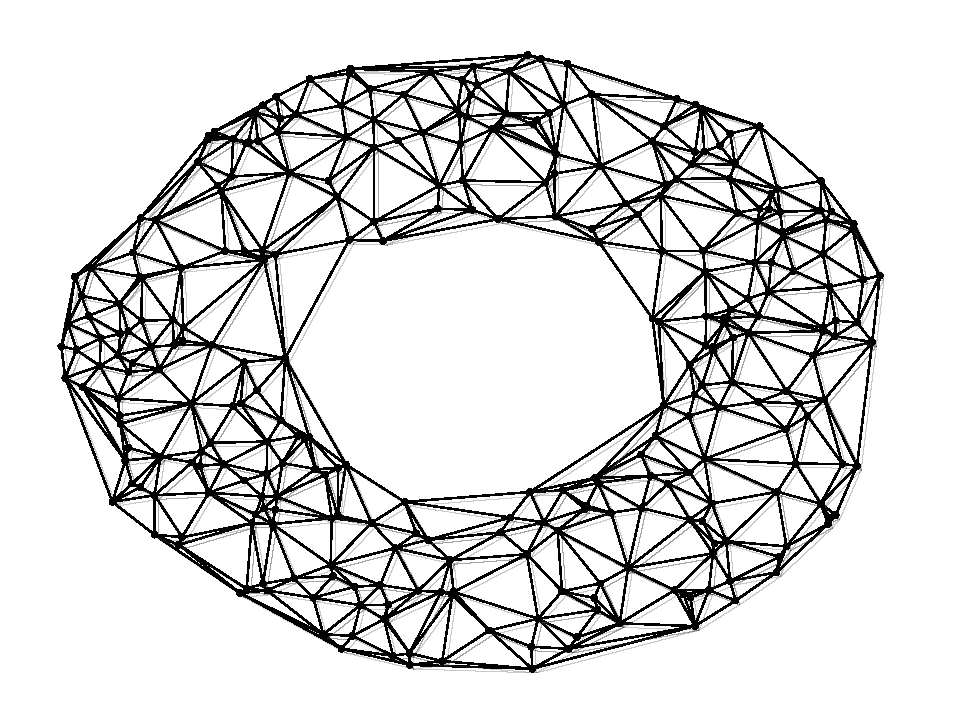
\includegraphics[scale=0.33]{figures/boundary_graph.pdf}
    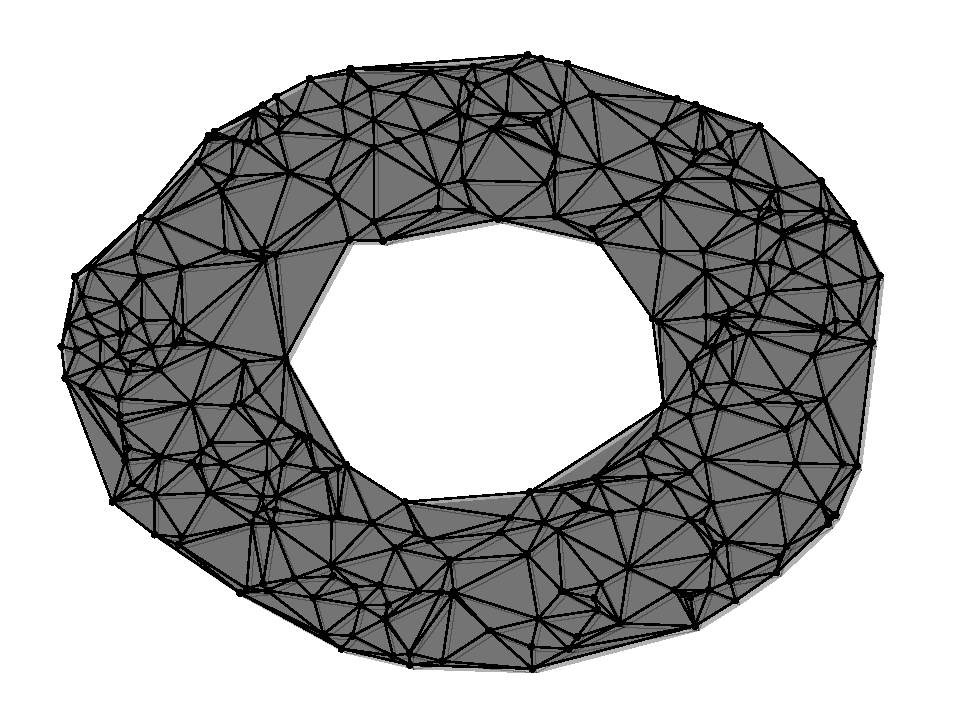
\includegraphics[scale=0.33]{figures/boundary_complex.pdf}
    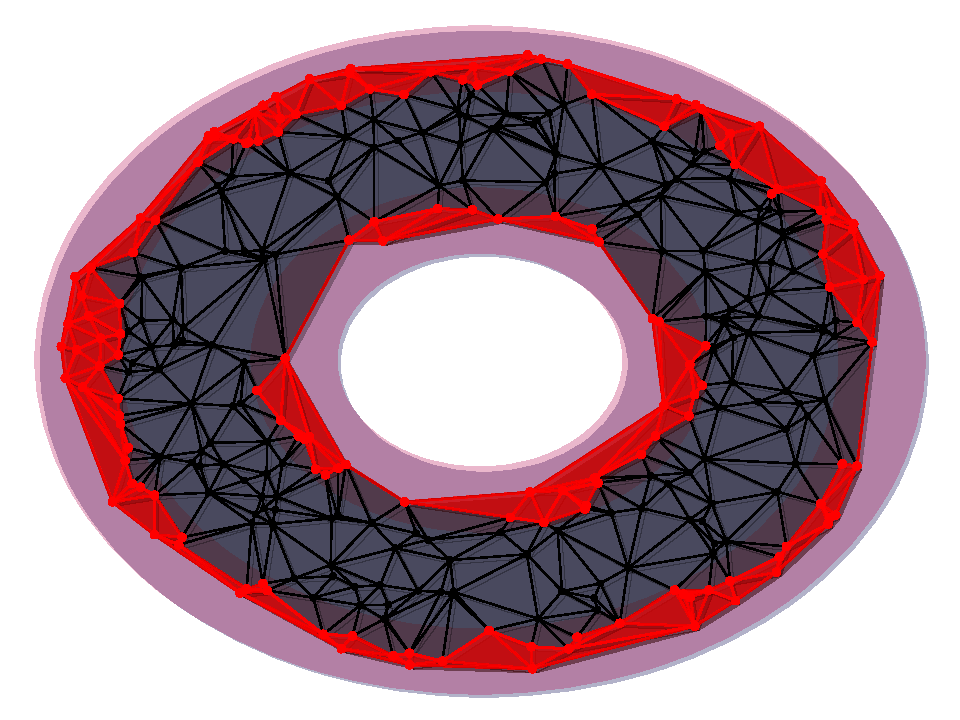
\includegraphics[scale=0.33]{figures/boundary_complex_domain_fence.pdf}
    % 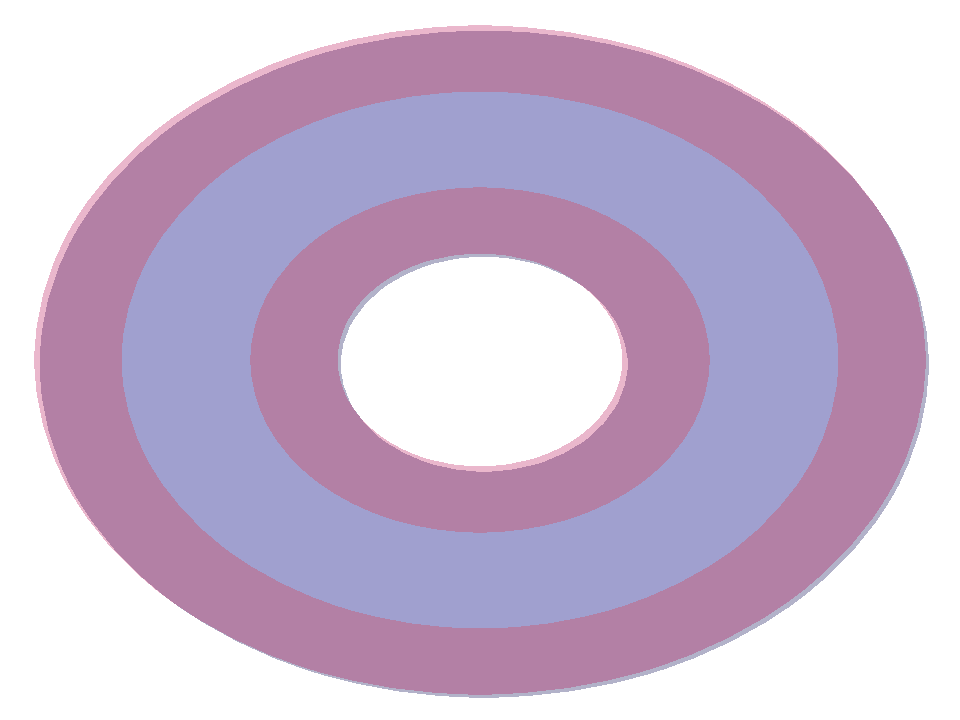
\includegraphics[scale=0.24]{figures/boundary_domain.pdf}
     \caption{(Left) The neighborhood graph of a sensor network with a large ``hole''.
            (Middle) A 2-dimensional simplicial complex with no gaps in coverage, but an unfilled cycle.
            (Right) By allowing nodes to identify the boundary (in red) we can confirm coverage of complex domains.}
     \label{fig:boundary1}
 \end{figure}

In order to \textit{verify} coverage by we need our network to sufficiently sample the extent of our domain.
Moreover, if there are gaps in coverage, are they due to insufficient sampling or a gap in the domain itself?
Let $\B\subset\D$ be the \textbf{boundary} of our domain and let our sensors detect whe the are within communication radius of $\B$.
Let $Q = \{p\in P\mid \min_{x\in\B}\dist(x, p)\}$ be the set of \textbf{boundary nodes} in $P$.
The set $Q$ induces a \textbf{subcomplex} $\rips^\alpha(Q)$ of $\rips^\alpha(K)$ restricted to nodes in $Q$.
% Assuming there are no holes in our network no path from a point in $P\setminus Q$ to a point outside our domain  without crossing a simplex in $K\mid_Q$.

% \textbf{TODO} Section overview.
% We will show how this construction is used to verify coverage of a specific subset of a bounded domain $\D$ with a tight bound on the coverage radius.

% Note that the communication radius is far from a tight bound on the coverage radius.

% section complexes (end)
